% Options for packages loaded elsewhere
\PassOptionsToPackage{unicode}{hyperref}
\PassOptionsToPackage{hyphens}{url}
%
\documentclass[
]{book}
\usepackage{lmodern}
\usepackage{amssymb,amsmath}
\usepackage{ifxetex,ifluatex}
\ifnum 0\ifxetex 1\fi\ifluatex 1\fi=0 % if pdftex
  \usepackage[T1]{fontenc}
  \usepackage[utf8]{inputenc}
  \usepackage{textcomp} % provide euro and other symbols
\else % if luatex or xetex
  \usepackage{unicode-math}
  \defaultfontfeatures{Scale=MatchLowercase}
  \defaultfontfeatures[\rmfamily]{Ligatures=TeX,Scale=1}
\fi
% Use upquote if available, for straight quotes in verbatim environments
\IfFileExists{upquote.sty}{\usepackage{upquote}}{}
\IfFileExists{microtype.sty}{% use microtype if available
  \usepackage[]{microtype}
  \UseMicrotypeSet[protrusion]{basicmath} % disable protrusion for tt fonts
}{}
\makeatletter
\@ifundefined{KOMAClassName}{% if non-KOMA class
  \IfFileExists{parskip.sty}{%
    \usepackage{parskip}
  }{% else
    \setlength{\parindent}{0pt}
    \setlength{\parskip}{6pt plus 2pt minus 1pt}}
}{% if KOMA class
  \KOMAoptions{parskip=half}}
\makeatother
\usepackage{xcolor}
\IfFileExists{xurl.sty}{\usepackage{xurl}}{} % add URL line breaks if available
\IfFileExists{bookmark.sty}{\usepackage{bookmark}}{\usepackage{hyperref}}
\hypersetup{
  pdftitle={A Minimal Book Example},
  pdfauthor={Yihui Xie},
  hidelinks,
  pdfcreator={LaTeX via pandoc}}
\urlstyle{same} % disable monospaced font for URLs
\usepackage{color}
\usepackage{fancyvrb}
\newcommand{\VerbBar}{|}
\newcommand{\VERB}{\Verb[commandchars=\\\{\}]}
\DefineVerbatimEnvironment{Highlighting}{Verbatim}{commandchars=\\\{\}}
% Add ',fontsize=\small' for more characters per line
\usepackage{framed}
\definecolor{shadecolor}{RGB}{248,248,248}
\newenvironment{Shaded}{\begin{snugshade}}{\end{snugshade}}
\newcommand{\AlertTok}[1]{\textcolor[rgb]{0.94,0.16,0.16}{#1}}
\newcommand{\AnnotationTok}[1]{\textcolor[rgb]{0.56,0.35,0.01}{\textbf{\textit{#1}}}}
\newcommand{\AttributeTok}[1]{\textcolor[rgb]{0.77,0.63,0.00}{#1}}
\newcommand{\BaseNTok}[1]{\textcolor[rgb]{0.00,0.00,0.81}{#1}}
\newcommand{\BuiltInTok}[1]{#1}
\newcommand{\CharTok}[1]{\textcolor[rgb]{0.31,0.60,0.02}{#1}}
\newcommand{\CommentTok}[1]{\textcolor[rgb]{0.56,0.35,0.01}{\textit{#1}}}
\newcommand{\CommentVarTok}[1]{\textcolor[rgb]{0.56,0.35,0.01}{\textbf{\textit{#1}}}}
\newcommand{\ConstantTok}[1]{\textcolor[rgb]{0.00,0.00,0.00}{#1}}
\newcommand{\ControlFlowTok}[1]{\textcolor[rgb]{0.13,0.29,0.53}{\textbf{#1}}}
\newcommand{\DataTypeTok}[1]{\textcolor[rgb]{0.13,0.29,0.53}{#1}}
\newcommand{\DecValTok}[1]{\textcolor[rgb]{0.00,0.00,0.81}{#1}}
\newcommand{\DocumentationTok}[1]{\textcolor[rgb]{0.56,0.35,0.01}{\textbf{\textit{#1}}}}
\newcommand{\ErrorTok}[1]{\textcolor[rgb]{0.64,0.00,0.00}{\textbf{#1}}}
\newcommand{\ExtensionTok}[1]{#1}
\newcommand{\FloatTok}[1]{\textcolor[rgb]{0.00,0.00,0.81}{#1}}
\newcommand{\FunctionTok}[1]{\textcolor[rgb]{0.00,0.00,0.00}{#1}}
\newcommand{\ImportTok}[1]{#1}
\newcommand{\InformationTok}[1]{\textcolor[rgb]{0.56,0.35,0.01}{\textbf{\textit{#1}}}}
\newcommand{\KeywordTok}[1]{\textcolor[rgb]{0.13,0.29,0.53}{\textbf{#1}}}
\newcommand{\NormalTok}[1]{#1}
\newcommand{\OperatorTok}[1]{\textcolor[rgb]{0.81,0.36,0.00}{\textbf{#1}}}
\newcommand{\OtherTok}[1]{\textcolor[rgb]{0.56,0.35,0.01}{#1}}
\newcommand{\PreprocessorTok}[1]{\textcolor[rgb]{0.56,0.35,0.01}{\textit{#1}}}
\newcommand{\RegionMarkerTok}[1]{#1}
\newcommand{\SpecialCharTok}[1]{\textcolor[rgb]{0.00,0.00,0.00}{#1}}
\newcommand{\SpecialStringTok}[1]{\textcolor[rgb]{0.31,0.60,0.02}{#1}}
\newcommand{\StringTok}[1]{\textcolor[rgb]{0.31,0.60,0.02}{#1}}
\newcommand{\VariableTok}[1]{\textcolor[rgb]{0.00,0.00,0.00}{#1}}
\newcommand{\VerbatimStringTok}[1]{\textcolor[rgb]{0.31,0.60,0.02}{#1}}
\newcommand{\WarningTok}[1]{\textcolor[rgb]{0.56,0.35,0.01}{\textbf{\textit{#1}}}}
\usepackage{longtable,booktabs}
% Correct order of tables after \paragraph or \subparagraph
\usepackage{etoolbox}
\makeatletter
\patchcmd\longtable{\par}{\if@noskipsec\mbox{}\fi\par}{}{}
\makeatother
% Allow footnotes in longtable head/foot
\IfFileExists{footnotehyper.sty}{\usepackage{footnotehyper}}{\usepackage{footnote}}
\makesavenoteenv{longtable}
\usepackage{graphicx,grffile}
\makeatletter
\def\maxwidth{\ifdim\Gin@nat@width>\linewidth\linewidth\else\Gin@nat@width\fi}
\def\maxheight{\ifdim\Gin@nat@height>\textheight\textheight\else\Gin@nat@height\fi}
\makeatother
% Scale images if necessary, so that they will not overflow the page
% margins by default, and it is still possible to overwrite the defaults
% using explicit options in \includegraphics[width, height, ...]{}
\setkeys{Gin}{width=\maxwidth,height=\maxheight,keepaspectratio}
% Set default figure placement to htbp
\makeatletter
\def\fps@figure{htbp}
\makeatother
\setlength{\emergencystretch}{3em} % prevent overfull lines
\providecommand{\tightlist}{%
  \setlength{\itemsep}{0pt}\setlength{\parskip}{0pt}}
\setcounter{secnumdepth}{5}
\usepackage{booktabs}
\usepackage{amsthm}
\makeatletter
\def\thm@space@setup{%
  \thm@preskip=8pt plus 2pt minus 4pt
  \thm@postskip=\thm@preskip
}
\makeatother
\usepackage[]{natbib}
\bibliographystyle{apalike}

\title{A Minimal Book Example}
\author{Yihui Xie}
\date{2020-01-10}

\begin{document}
\frontmatter
\maketitle

{
\setcounter{tocdepth}{1}
\tableofcontents
}
\mainmatter
\hypertarget{prerequisites}{%
\chapter{Prerequisites}\label{prerequisites}}

This is a \emph{sample} book written in \textbf{Markdown}. You can use anything that Pandoc's Markdown supports, e.g., a math equation \(a^2 + b^2 = c^2\).

The \textbf{bookdown} package can be installed from CRAN or Github:

\begin{Shaded}
\begin{Highlighting}[]
\KeywordTok{install.packages}\NormalTok{(}\StringTok{"bookdown"}\NormalTok{)}
\CommentTok{# or the development version}
\CommentTok{# devtools::install_github("rstudio/bookdown")}
\end{Highlighting}
\end{Shaded}

Remember each Rmd file contains one and only one chapter, and a chapter is defined by the first-level heading \texttt{\#}.

To compile this example to PDF, you need XeLaTeX. You are recommended to install TinyTeX (which includes XeLaTeX): \url{https://yihui.name/tinytex/}.

\hypertarget{course-description}{%
\chapter{Course Description}\label{course-description}}

PQHS 432 (cross-listed as CRSP 432 and MPHP 432, and formerly known as EPBI 432) is the second half of a two-semester sequence (with PQHS 431) focused on modern data analysis and advanced statistical modeling, with a practical bent (as little theory as possible), emphasizing the key role of thinking hard, and well, about design and analysis in research. The title listed by the registrar is a little dated - I prefer \emph{Data Science for Biological, Medical or Health Research}.

This is a good course for people who want to learn how to use the R language to get information from data, and who want to learn about making comparisons and building models to help make meaningful progress in research, focusing on questions from biology, medicine and public health. We spend time managing and visualizing data, building models and making predictions, and other things thought of as ``data science'' - in essence, this highly applied course focuses on modern, more than classical, tools for learning from data. The course is taught using the R statistical software and RStudio environments, with the material discussed in 431 assumed in 432. Students learned a lot of R in the 431 course, and that material remains available at \url{https://github.com/THOMASELOVE/2019-431}. We'll continue to use R Studio and R Markdown as tools to help make R work better, and perform our research in replicable ways.

\hypertarget{general-approach-topics}{%
\section{General Approach / Topics}\label{general-approach-topics}}

The course covers the following general topics, roughly in this order, through early April. Additional topics (for the remainder of April) will be determined later in the semester.

\begin{enumerate}
\def\labelenumi{\arabic{enumi}.}
\tightlist
\item
  Linear Regression (including weighted and robust approaches, variable selection, dealing with missing data, fitting non-linear relationships through predictor transformation, cross-validation approaches, and multi-factor ANOVA and ANCOVA)
\item
  Logistic Regression (including both models for binary outcomes, and models for proportions, and risk adjustment)
\item
  Generalized Linear Models (including regression models for count data, multi-categorical outcomes)
\item
  The Statistical Crisis in Science
\item
  Cluster Analysis (mostly in the form of Principal Components Analysis)
\item
  Survival Analysis (Kaplan-Meier curves and Cox Regression)
\end{enumerate}

\hypertarget{prerequisites-1}{%
\section{Prerequisites}\label{prerequisites-1}}

Taking 432 without 431 is not recommended. The pace can be brisk at times, but all CWRU students who feel up to it are welcome, in any field of study.

The main things students need for 432 are:

\begin{itemize}
\tightlist
\item
  tools: substantive knowledge of the use of R, R Studio and R Markdown to produce code which will ingest, visualize, explore, analyze and model data, then communicate the results
\item
  statistical methodology: substantive understanding of statistical inference in the one-, two- and multi-sample cases and the fundamentals of linear regression models, including the building of multiple linear regressions, and their evaluation through diagnostic plots, stepwise model selection, assessment of uncertainty via confidence and prediction intervals, and basic in-sample and out-of sample validation summaries
\item
  data to study related to biological, health, medical, scientific or other phenomena, and
\item
  an interest in studying data closely and presenting rigorous analyses effectively
\end{itemize}

Some of these topics are reviewed in early 432 sessions.

\hypertarget{everything-is-on-the-web}{%
\section{Everything is on the Web}\label{everything-is-on-the-web}}

\url{https://github.com/THOMASELOVE/2020-432} is the place to go for everything related to this course. Please visit any time you need something. I update the web site frequently.

\begin{itemize}
\tightlist
\item
  The most important thing is the \href{https://github.com/THOMASELOVE/2020-432/blob/master/calendar.md}{Course Calendar} which serves as the final word for all deadlines, plus links to all classes and deliverables.
\item
  Dr.~Love's \href{https://thomaselove.github.io/2020-432-book/}{book of 432 Course Notes} is the principal textbook for the course, and will appear during the semester. The \href{https://thomaselove.github.io/2019-432-book/}{Spring 2019 version} is available now.
\end{itemize}

Additional details will be coming soon.

\hypertarget{professor-love}{%
\chapter{Professor Love}\label{professor-love}}

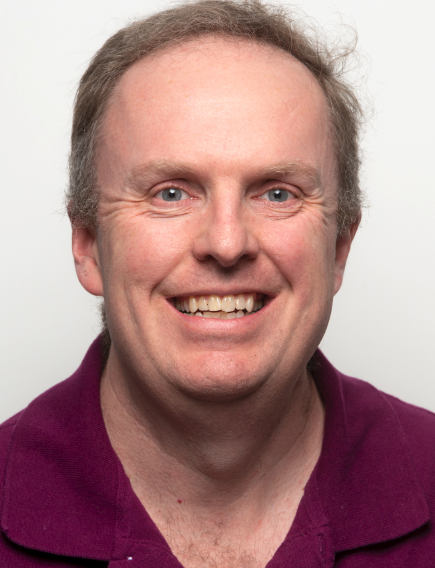
\includegraphics[width=0.3\linewidth]{figures/Love2019}

Thomas E. Love, Ph.D.

\begin{itemize}
\tightlist
\item
  Professor of Medicine, Population and Quantitative Health Sciences, \href{http://case.edu/}{CWRU}
\item
  Director of \href{http://chrp.org/biostatistics-evaluation/}{Biostatistics and Evaluation}, \href{http://chrp.org/}{Center for Health Care Research \& Policy}, \href{https://www.metrohealth.org/research}{MetroHealth Medical Center}
\item
  \href{http://www.betterhealthpartnership.org/data_center/}{Chief Data Scientist}, \href{http://betterhealthpartnership.org/}{Better Health Partnership}
\item
  Track Lead for Health Care Analytics, MS in Biostatistics, \href{http://epbiwww.case.edu/}{Department of Population and Quantitative Health Sciences}, CWRU
\item
  Fellow, \href{http://www.amstat.org/}{American Statistical Association}
\end{itemize}

\hypertarget{a-more-complete-biography}{%
\section{A More Complete Biography}\label{a-more-complete-biography}}

Hi. I am Thomas E. Love, Ph.D.~and I have at least three different jobs.

\begin{itemize}
\tightlist
\item
  I am a Professor in the Departments of Medicine and Population \& Quantitative Health Sciences at Case Western Reserve University. I teach three courses per year there (PQHS 431, 432 and 500) and also lead the Health Care Analytics track of the MS program in Biostatistics.
\item
  I direct \href{http://chrp.org/biostatistics-evaluation/}{Biostatistics and Evaluation} at the \href{http://chrp.org/}{Center for Health Care Research \& Policy}, which is a joint venture of CWRU and MetroHealth Medical Center.
\item
  For ten years, I was the (founding) Data Director for \href{http://betterhealthpartnership.org/}{Better Health Partnership}, an alliance of people who provide, pay for and receive care in Northeast Ohio. I now serve as Chief Data Scientist there.
\item
  I am a Fellow of the American Statistical Association, and have won numerous awards for my teaching and my research, including the 2018 \href{https://students.case.edu/traditions/awards/diekhoff/}{John S. Diekhoff Award for Graduate Teaching} from CWRU.
\item
  I have been teaching at CWRU since 1994, and have taught every manner of CWRU student over the years, especially students in biostatistics, medicine, and management.
\end{itemize}

In research, I use statistical methods to look at questions in health policy and in particular the provision of health services. I mostly work with observational data, rather than data that emerge from randomized clinical trials, and I have a special interest in working with data from electronic health records.

\begin{itemize}
\tightlist
\item
  You may be interested in a \href{http://content.healthaffairs.org/content/34/7/1121.abstract}{recent study in Health Affairs} showing the impact of a \href{http://thedaily.case.edu/new-study-shows-prepared-safety-net-improves-care-saves-money-in-medicaid-expansion-population/}{Medicaid-like expansion plan on care and outcomes of poor patients in Cleveland}.
\item
  Or you might be interested in our \href{http://www.nejm.org/doi/full/10.1056/NEJMsa1102519}{New England Journal of Medicine study} of the effect of electronic health records on the care and outcomes of people with diabetes.
\item
  In 2011, \href{http://tdi.dartmouth.edu/faculty/a-james-omalley-phd}{James O'Malley} and I chaired the \href{https://ww2.amstat.org/meetings/ichps/2011/index.cfm?fuseaction=main}{Ninth International Conference on Health Policy Statistics}, here in Cleveland. Here's a \href{https://link.springer.com/article/10.1007\%2Fs10742-012-0096-8}{recap}.
\item
  I've also worked on many projects involving the use of propensity scores to make causal inferences from observational studies, particularly in heart failure.
\end{itemize}

If you want to see a \href{https://www.ncbi.nlm.nih.gov/myncbi/thomas.love.1/bibliography/public/}{pretty complete list of my publications}, knock yourself out.

I hold degrees from Columbia University in the City of New York and from the University of Pennsylvania. My dissertation adviser was Paul Rosenbaum. I am married to a brilliant woman who is an attorney at GE Lighting, and we are raising two terrific sons. The elder is a junior in college (University of Pittsburgh) who plans to be a paleontologist, and one finishing high school this year, who will attend Columbia this Fall. I live in Shaker Heights. I also sing and act occasionally in \href{https://github.com/THOMASELOVE/theater}{community theater}.

\hypertarget{email}{%
\section{Email}\label{email}}

\begin{itemize}
\tightlist
\item
  Email to get help with the course: \textbf{431-help at case dot edu} (seen by Professor Love and the TAs)
\item
  \texttt{Thomas\ dot\ Love\ at\ case\ dot\ edu} (for matters related to grades or individual concerns)
\item
  Professor Love is hard to reach by phone. Email is always the best way to reach him.
\end{itemize}

\hypertarget{offices}{%
\section{Offices}\label{offices}}

\begin{itemize}
\tightlist
\item
  Wood WG-82J on the ground floor of the Wood building (Tuesdays and Thursdays)
\item
  Rammelkamp R-229A at MetroHealth Medical Center (Wednesdays and Fridays)
\end{itemize}

Professor Love is available for the 15 minutes before and the 30 minutes after each class, and otherwise by appointment on Tuesdays and Thursdays (send email to schedule).

\hypertarget{name-and-pronouns}{%
\section{Name and Pronouns}\label{name-and-pronouns}}

\begin{itemize}
\tightlist
\item
  Professor Love uses he/him/his pronouns.
\item
  Most students refer to him either as Professor Love or Dr.~Love.
\item
  He prefers his given name to be written ``Thomas'' as opposed to ``Tom''.
\item
  Most of his friends and colleagues call him ``Tom''. You are welcome to do so, as well, if that makes you more comfortable.
\end{itemize}

\hypertarget{web}{%
\section{Web}\label{web}}

\begin{itemize}
\tightlist
\item
  Professor Love's \href{https://thomaselove.github.io/}{GitHub pages website}.

  \begin{itemize}
  \tightlist
  \item
    His GitHub name is \href{https://github.com/thomaselove}{THOMASELOVE}.
  \end{itemize}
\item
  His Twitter handle is \href{https://twitter.com/ThomasELove}{ThomasELove}.
\end{itemize}

\hypertarget{teaching-assistants}{%
\chapter{Teaching Assistants}\label{teaching-assistants}}

\begin{itemize}
\tightlist
\item
  To contact the TAs (and Dr.~Love) at any time, email \texttt{431-help} at \texttt{case\ dot\ edu}.
\end{itemize}

The teaching assistants for 432 this year are

\begin{itemize}
\tightlist
\item
  {[}Benjamin Booker, BS{]}
\item
  \protect\hyperlink{julijana-conic-md}{Julijana Conic, MD}
\item
  \protect\hyperlink{joseph-hnath-ba}{Joseph Hnath, BA}
\item
  \protect\hyperlink{amr-mahran-md-ms}{Amr Mahran, MD MS}
\item
  \protect\hyperlink{amin-saad-md}{Amin Saad, MD}
\end{itemize}

They are the people answering \texttt{431-help\ at\ case\ dot\ edu}, and they are the people holding the bulk of our regular office hours. Most of them has been in your shoes - they've taken the course in the past, and they enjoyed it enough to come back for more. Many have volunteered their precious time and energy to help make the course happen, and we couldn't be more delighted to welcome you to the course. To contact the TAs, email \texttt{431-help\ at\ case\ dot\ edu}, which is open all semester, starting on the first day we meet.

\hypertarget{office-hours-for-tas}{%
\section{Office Hours for TAs}\label{office-hours-for-tas}}

\begin{itemize}
\tightlist
\item
  To contact the TAs (and Dr.~Love) at any time, email \texttt{431-help} at \texttt{case\ dot\ edu}. This is a challenging class. Don't suffer in silence - talk to us!
\end{itemize}

Teaching Assistant Office Hours are held in either WG-56 (Computing Lab) or WG-67 (Student Lounge) on the ground floor of the Wood building in the School of Medicine, so be sure to look in both places if you need help. The weekly schedule will be posted on the bottom of the \href{https://github.com/THOMASELOVE/2020-432/blob/master/calendar.md}{Course Calendar}.

TA office hours are not held on University holidays, or during Spring Break, although 431-help remains open until the last project is completed in May.

This is a challenging class. Don't suffer in silence - talk to us!

\hypertarget{benjamin-ben-booker-bs}{%
\section{Benjamin (Ben) Booker, BS}\label{benjamin-ben-booker-bs}}


\includegraphics[width=0.3\linewidth]{figures/Ben}

Benjamin (Ben) Booker is a first year PhD student in the Epidemiology \& Biostatistics program in the Department of Population \& Quantitative Health Sciences. Ben holds a BS in Molecular Biology from the University of Cincinnati, and then completed two years of additional training in Biostatistics there. He has worked at Cincinnati Children's Hospital performing DNA methylation analysis, and as a data scientist consultant for Givaudan Flavors. Outside of work and school I enjoy rock climbing/bouldering (novice level), playing soccer and watching the European football leagues.

\hypertarget{julijana-conic-md}{%
\section{Julijana Conic, MD}\label{julijana-conic-md}}

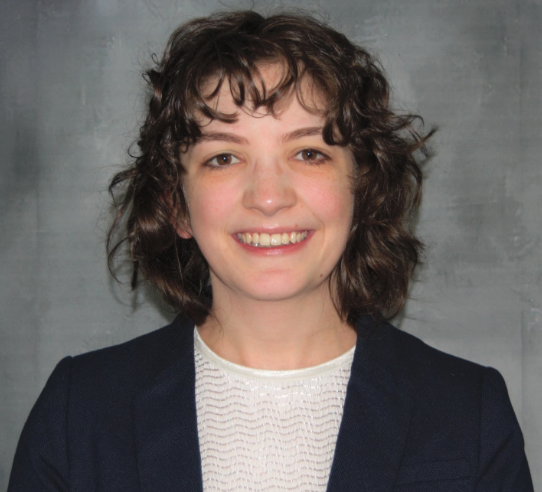
\includegraphics[width=0.3\linewidth]{figures/Julijana}

Julijana Conic was born in Serbia and received her MD from the University of Belgrade Faculty of Medicine last year. Since enrolling in the MS in Clinical Research program the same year she has been conducting research focusing on ischemic mitral regurgitation in the Department of Cardiovascular Imagining at the Cleveland Clinic. Currently, she is working on a project incorporating machine learning to improve existing algorithms for automatic quantification of cardiac volumes on MRI images and to aid in risk stratification of ischemic mitral regurgitation patients. She hopes to start internal medicine residency next year and ultimately establish herself as a physician investigator. During her free time Julijana enjoys hiking, watching movies and volunteering in the community.

\hypertarget{joseph-hnath-ba}{%
\section{Joseph Hnath, BA}\label{joseph-hnath-ba}}

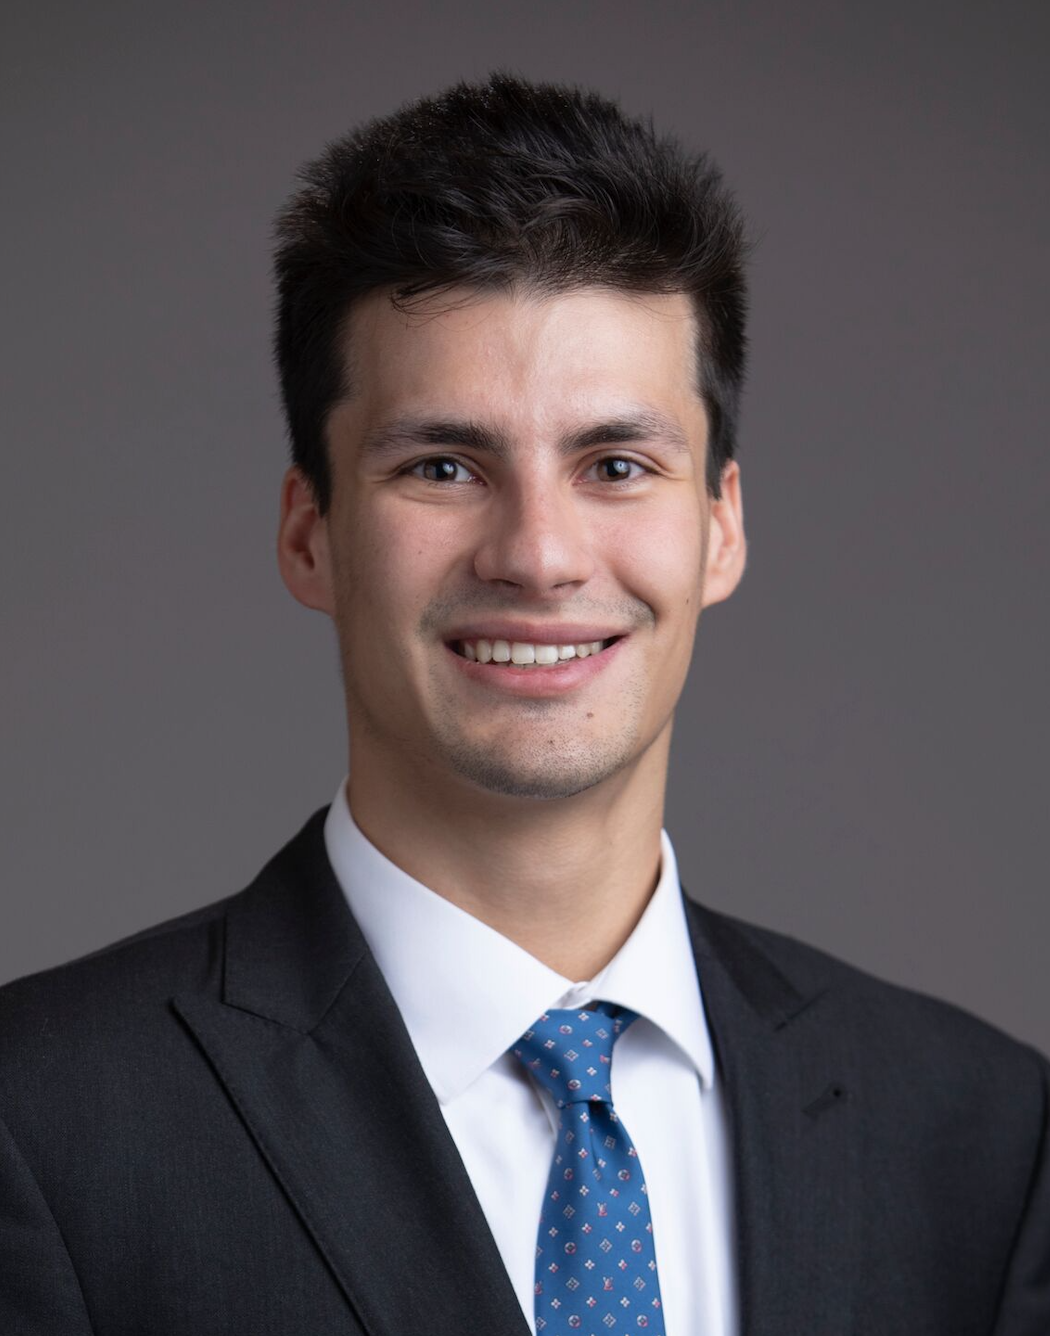
\includegraphics[width=0.3\linewidth]{figures/Joseph}

Joseph Hnath is in his second year of the Master of Public Health program on the Intensive Research Pathway with concentrations in Population Health Research and Health Policy \& Management. He finished his undergraduate studies at CWRU this May where he majored in Chemical Biology, Cognitive Science, and Economics. Having taken 431 \& 432 last year, the skills he learned have been invaluable in his research projects, such as his capstone on the health economics of abortion policy and helping with the NEO-CASE cancer disparities resource. Joseph enjoys playing basketball, watching Master Chef, and reading \emph{The Complete Works of F. Scott Fitzgerald}.

\hypertarget{amr-mahran-md-ms}{%
\section{Amr Mahran, MD MS}\label{amr-mahran-md-ms}}

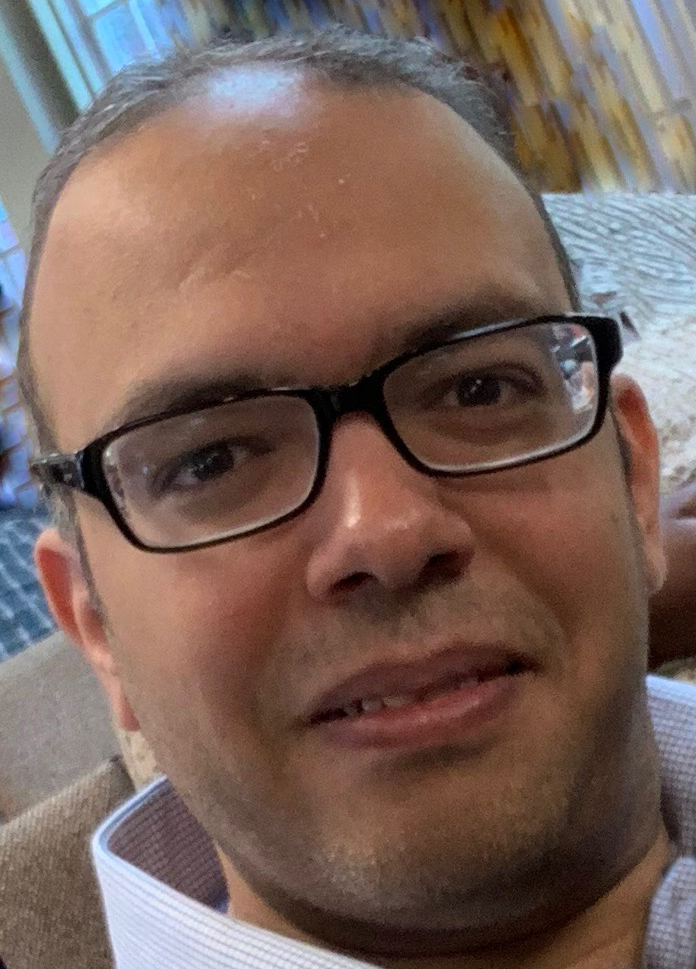
\includegraphics[width=0.3\linewidth]{figures/Amr}

Amr Mahran is a urologist who is working as a senior research associate in the department of urology, CWRU School of Medicine. He received his MD degree from Assiut University School of Medicine in Upper Egypt. He also finished a residency in urology along with earning a Master of Science degree. Before joining CWRU, Amr was a practicing urologist and was appointed as a faculty at the department of urology, Assiut University Hospitals. Amr took 432 in the spring of 2019 and learned many skills that helped him in his clinical research. Amr's research focus on prostate cancer, pelvic pain, and voiding dysfunction. He does outcome research on large databases as NSQIP, National Trauma Database (NTDB), and NIS databases. Amr enjoys playing soccer, table tennis, and reading.

\hypertarget{amin-saad-md}{%
\section{Amin Saad, MD}\label{amin-saad-md}}

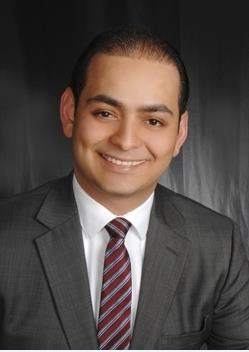
\includegraphics[width=0.3\linewidth]{figures/Amin}

Amin Saad is an international medical graduate from Syria with two years of General Surgery residency training experience in the United States. Amin is currently enrolled in the CRSP Master's program and is seeking a Ph.D.~degree in Clinical and Translational Research with a focus toward lowering surgical site infection rates. Amin took 431 and 432 two cycles ago and has appreciated how the skills he learned in those classes have helped him with his clinical outcomes research at the Department of Colorectal Surgery at University Hospitals. Amin enjoys playing soccer, swimming, and spending time with his family.

\hypertarget{deliverables-and-grading}{%
\chapter{Deliverables and Grading}\label{deliverables-and-grading}}

This section of the syllabus will appear soon.

\hypertarget{a-few-writingpresenting-tips}{%
\chapter{A Few Writing/Presenting Tips}\label{a-few-writingpresenting-tips}}

\begin{enumerate}
\def\labelenumi{\arabic{enumi}.}
\item
  Statistics is a ``getting the details right'' business - we care deeply about details, and this applies to writing code or complete English sentences.
\item
  Nothing impresses us as much as a clear and concise argument, presented using well-written English sentences, effective and well-labeled figures and tables.
\item
  Don't parrot back material that Dr.~Love wrote or said. State ideas in your own words. Stating them in other words is, technically, plagiarism.
\item
  Edit your more adventurous output; don't present everything you know how to do in R, and don't forget that someone is trying to read both your code and your results.
\item
  Make your work easy to evaluate. In responding to an assignment, be sure to answer the question that was asked, restating it as necessary.
\item
  Clearly label everything: graphs, tables, your answer to a specific question. Everything. Again, make your work easy to evaluate.
\item
  Simplify. Emphasize ideas in plain language. Avoid jargon. Use English well.
\item
  Data are plural. Use ``the data \textbf{are} \ldots{}'' rather than ``the data \emph{is} \ldots{} ''
\item
  A paragraph must contain more than one sentence.
\item
  Don't switch tenses. If you want to write in the present tense, stick to it throughout.
\item
  Don't write or say random sample unless you used a random number generator. If you used haphazard sampling or convenience sampling, call it what it is, and indicate whether any problems could have cropped up as a result.
\item
  Similarly, don't defend a method of data collection because it is random. Most of the time we want to represent some population, and a random sample is just one way to ensure that certain types of biases have a low probability of creeping in.
\item
  If you want to write that you used \(\alpha = 0.05\) as your significance level, then state that your results were obtained using a 95\% confidence level, not a 95\% confidence interval, unless you are actually interpreting a confidence interval.
\item
  If you're looking at a \emph{p}-value, then you should state either:

  \begin{itemize}
  \tightlist
  \item
    {[}1{]} We're using a 95\% confidence level.\\
  \item
    {[}2{]} We're using a 5\% significance level. or
  \item
    {[}3{]} We're using \(\alpha = 0.05\).\\
  \item
    Don't use more than one of these expressions.
  \end{itemize}
\item
  Refer to all \emph{p}-values that are less than 0.001 or perhaps less than 0.0001 as \(p < 0.001\), rather than, for instance, \(p = 0.00000001\) or, worse yet, \(p = 0\). In a similar vein, write all \(p\)-values that exceed 0.99 as \(p > 0.99\) instead of, for instance, \(p = 1\).
\item
  To the extent possible, don't use \texttt{computer-ese} to label variables, plots or tables. R and Markdown allow you to change the labels on graphs and tables to meaningful things -- do so. Use meaningful abbreviations, as necessary, explaining what they mean on the first usage.
\item
  Use words that we all know, whenever possible, and provide clear definitions at the first encounter when jargon is mandatory.
\item
  Often the most useful thing you can do in an analysis is to turn a table into a meaningful graph.
\item
  When in doubt, err on the side of clearer expression. Clear thinking causes and is demonstrated by clear writing.
\item
  In the words of \href{https://twitter.com/kjspin7/status/886006382993915904}{Edward Tufte}, to think clearly, keep asking yourself \ldots{}
\end{enumerate}

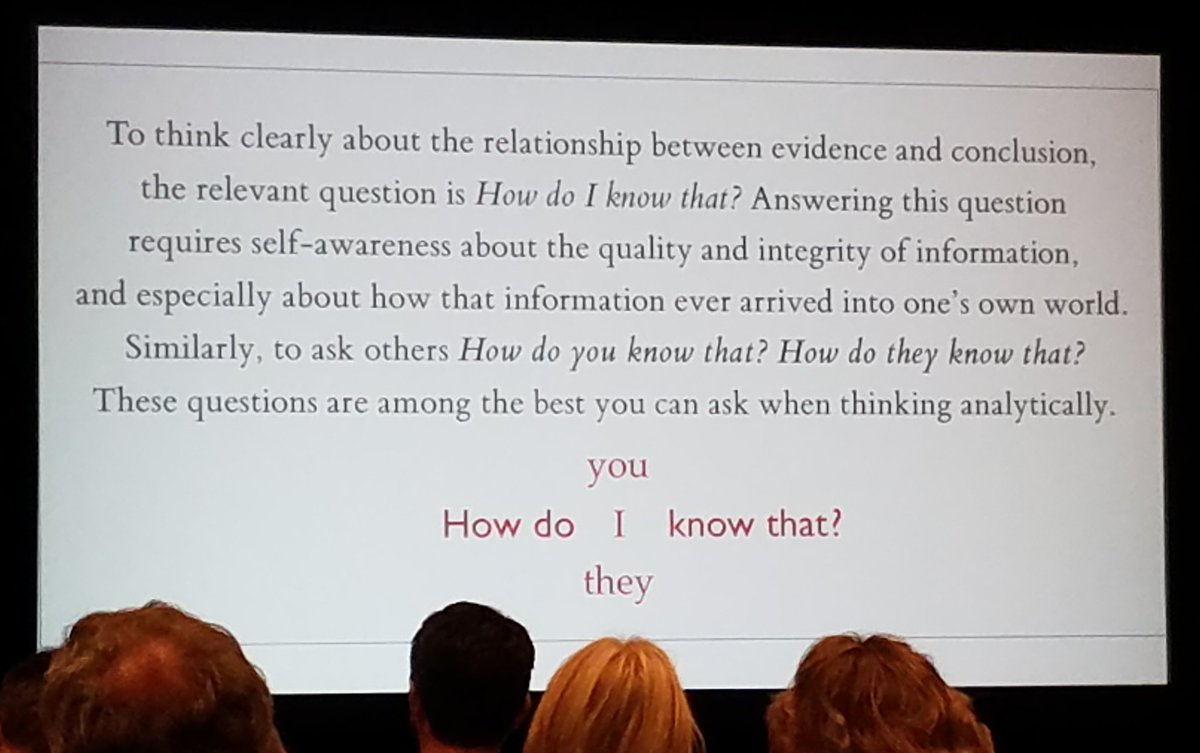
\includegraphics[width=0.85\linewidth]{figures/Tuftequote}

\backmatter
  \bibliography{book.bib,packages.bib}

\end{document}
